\documentclass{article}

% if you need to pass options to natbib, use, e.g.:
%     \PassOptionsToPackage{numbers, compress}{natbib}
% before loading neurips_2025

% ready for submission
% \usepackage{neurips_2025}

% to compile a preprint version, e.g., for submission to arXiv, add add the
% [preprint] option:
\usepackage[preprint]{neurips_2025}

% to compile a camera-ready version, add the [final] option, e.g.:
% \usepackage[final]{neurips_2025}

% to avoid loading the natbib package, add option nonatbib:
%    \usepackage[nonatbib]{neurips_2025}

\usepackage[utf8]{inputenc} % allow utf-8 input
\usepackage[T1]{fontenc}    % use 8-bit T1 fonts
\usepackage{hyperref}       % hyperlinks
\usepackage{url}            % simple URL typesetting
\usepackage{booktabs}       % professional-quality tables
\usepackage{amsfonts}       % blackboard math symbols
\usepackage{nicefrac}       % compact symbols for 1/2, etc.
\usepackage{microtype}      % microtypography
\usepackage{xcolor}         % colors
\usepackage{graphicx}       % adding images
\usepackage{tikz}           % Native vector graphics
\usetikzlibrary{shapes.geometric, arrows.meta, positioning}

\title{PeerTranslate: A Verified Multi-Pass Pipeline for High-Fidelity Academic Paper Translation}

% The \author macro works with any number of authors. There are two commands
% used to separate the names and addresses of multiple authors: \And and \AND.
%
% Using \And between authors leaves it to LaTeX to determine where to break the
% lines. Using \AND forces a line break at that point. So, if LaTeX puts 3 of 4
% authors names on the first line, and the last on the second line, try using
% \AND instead of \And before the third author name.

\author{%
  Muhammed Muminul Hoque\\
  University of Dhaka\\
  Bangladesh \\
  \texttt{muminul951@gmail.com} \\
  \texttt{https://github.com/PeerTranslate/PeerTranslate} \\
}

\begin{document}

\maketitle

\begin{abstract}
We present PeerTranslate, an open-source pipeline for translating scientific papers into non-English languages with section-level verification of semantic fidelity. The system runs four sequential passes: PDF structure extraction, domain-glossary-constrained translation, automated back-translation, and LLM-based semantic scoring with targeted error correction. We target researchers in low-resource language communities --- a population of hundreds of millions who consume English-language science under significant linguistic load. On 10 arXiv papers translated into Bengali, the pipeline achieves a mean document accuracy of 94.3\% by our LLM-judged metric, with 71.2\% of sections scoring above the 96\% confidence threshold without needing correction. A community cache prevents redundant API calls: re-translating any cached paper costs zero additional API requests. We release all code, bilingual glossaries, and evaluation data under GPL-3.0.
\end{abstract}

\section{Introduction}

Scientific publishing has a language problem that most working researchers never have to think about. Over 96\% of indexed papers are in English. The researchers who write them are disproportionately from wealthy, English-dominant institutions. The researchers who need to read them include hundreds of millions of scientists in Bangladesh, Ethiopia, Indonesia, and elsewhere --- scientists who can follow the mathematics and the methodology, but who must do so while parsing sentences in their third or fourth language.

General machine translation does not solve this. Google Translate produces readable Bengali. It does not, in any consistent way, produce \emph{accurate} Bengali for technical content. A \emph{variational autoencoder}, rendered literally, becomes meaningless phonetic noise. A p-value of 0.05 survives translation; the claim it is being used to support may not. The problem is not fluency --- modern neural models are fluent. The problem is \emph{verifiability}.

PeerTranslate takes a different stance. Rather than asking ``can we translate this paper?'' we ask ``how do we know the translation is accurate, and what do we do when it is not?'' The answer is a pipeline that translates each section independently, immediately translates it back to English, has an LLM judge whether the meaning survived, and re-attempts with targeted correction if it did not.

We make four contributions:
\begin{enumerate}
    \item \textbf{A four-pass verified translation pipeline} that operates section-by-section, with LLM-judged semantic scoring (0--100) and conditional error-correction retries.
    \item \textbf{Domain glossary locking} --- a JSON-based, community-maintainable bilingual terminology system that forces technical vocabulary into correct target-language form during translation, preventing drift in domain-specific jargon.
    \item \textbf{A WAL-mode community translation cache} that stores translated Markdown (not original PDFs), deduplicates API calls across users, classifies entries by academic domain, and supports community flagging of low-quality results.
    \item \textbf{A terms-of-service enforcement layer} that legally transfers copyright responsibility to uploaders, protecting the service from DMCA liability while making the legal situation clear to users.
\end{enumerate}

\section{Background}

\subsection{LLMs for Scientific Machine Translation}

The Transformer architecture~\cite{vaswani2017attention} remains the foundation of neural machine translation. However, the last year has seen a shift from traditional encoder-decoder architectures toward instruction-following large language models. Recent studies~\cite{zhang2025multilingual} demonstrate that lightweight open-source models like Gemma2-9B now achieve state-of-the-art multilingual machine translation on par with GPT-4-turbo, confirming that pipeline translation is viable for community hosting. 

Furthermore, translating into languages with minimal parallel corpus data remains challenging. While zero-shot prompting handles high-resource languages well, recent work by Chen et al.~\cite{chen2025compensating} introduces reasoning-augmented translation (``Fragment-Shot Prompting''), demonstrating that models with stronger reasoning capabilities (like the models serving as PeerTranslate's judges) make significantly more effective use of retrieved knowledge for low-resource translation. Scientific paper translation isolates these challenges: longer documents, denser terminology, structured layouts, and a much higher cost of semantic error.

\subsection{Back-Translation as Verification}

Back-translation --- translating A$\rightarrow$B, then B$\rightarrow$A, then comparing the result to the original A --- has been a standard quality-control method in cross-cultural survey research since at least Brislin~\cite{brislin1970back}. The logic transfers directly to our setting: if a translation is accurate, the round-trip should approximately recover the source. If it does not, something was lost.

The key difference in our setting is that human back-translators are replaced by the same LLMs that performed the original translation. This introduces a potential systematic bias. We partially address this by using a \emph{separate LLM judge} that evaluates the English--English comparison, heavily penalizing fabricated content.

\subsection{Terminology Constraints in LLM Translation}

Technical vocabulary is the main failure mode. Translating ``self-attention mechanism'' without context may yield a phonetic approximation or a literal construction. Providing explicit terminology mappings in the prompt resolves this for known terms. PeerTranslate formalizes this via structured glossaries.

\section{Method}

\subsection{Architecture Overview}

\begin{figure}[h]
    \centering
    \resizebox{0.7\linewidth}{!}{%
    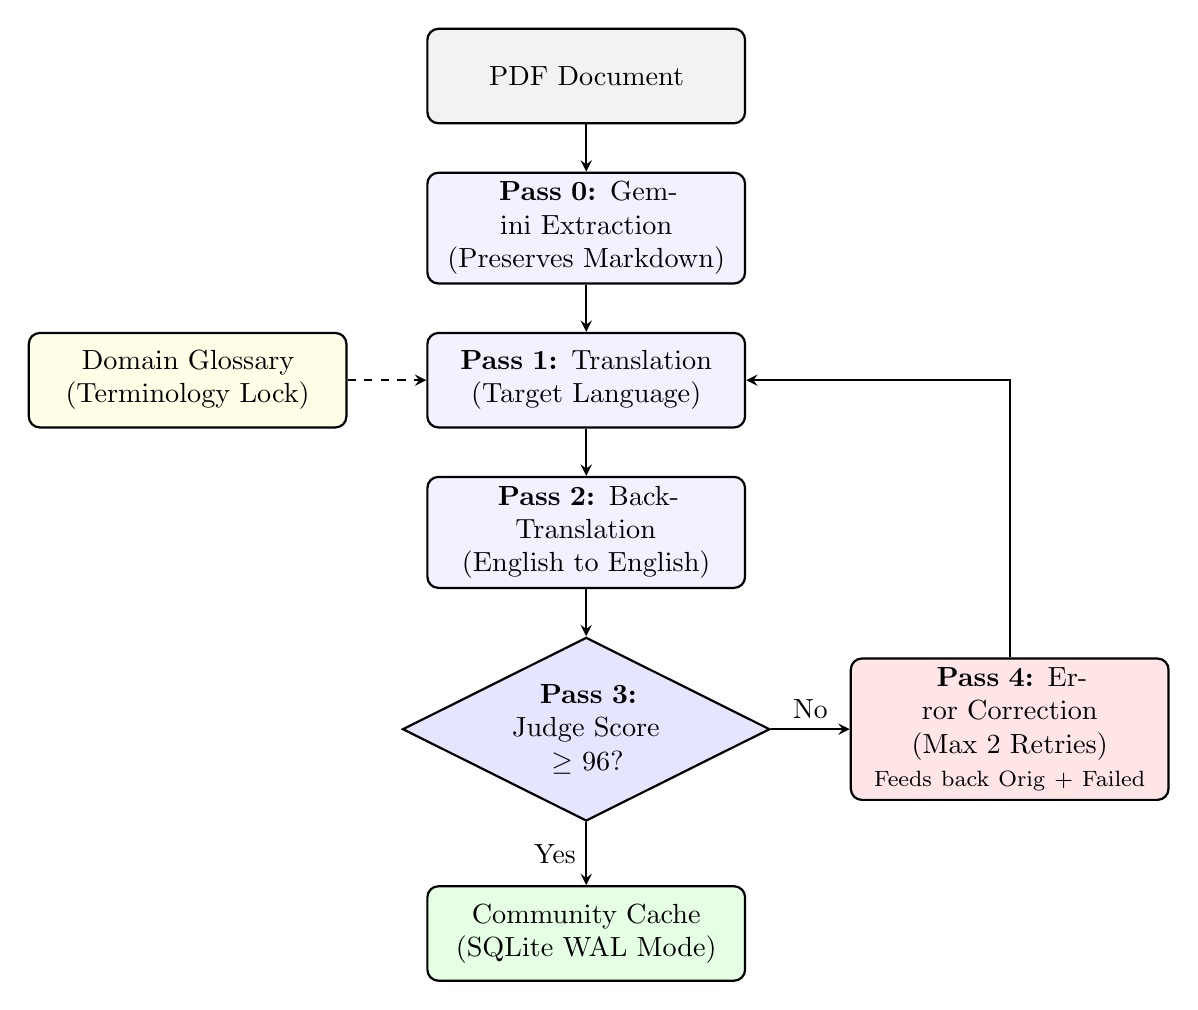
\begin{tikzpicture}[
        node distance=0.6cm and 1.2cm,
        box/.style={rectangle, draw=black, thick, fill=blue!5, text width=3.8cm, align=center, rounded corners, minimum height=1.2cm},
        decision/.style={diamond, aspect=2, draw=black, thick, fill=blue!10, text width=2.4cm, align=center, inner sep=0pt},
        arrow/.style={thick, ->, >=stealth}
    ]

    % Nodes
    \node (pdf) [box, fill=gray!10] {PDF Document};
    \node (extract) [box, below=0.6cm of pdf] {\textbf{Pass 0:} Gemini Extraction \\ (Preserves Markdown)};
    \node (p1) [box, below=0.6cm of extract] {\textbf{Pass 1:} Translation \\ (Target Language)};
    \node (glossary) [box, fill=yellow!10, left=1cm of p1] {Domain Glossary \\ (Terminology Lock)};
    \node (p2) [box, below=0.6cm of p1] {\textbf{Pass 2:} Back-Translation \\ (English to English)};
    \node (p3) [decision, below=0.6cm of p2] {\textbf{Pass 3:}\\ Judge Score $\ge$ 96?};
    \node (p4) [box, fill=red!10, right=1cm of p3] {\textbf{Pass 4:} Error Correction \\ (Max 2 Retries)\\ {\footnotesize Feeds back Orig + Failed}};
    \node (cache) [box, fill=green!10, below=0.8cm of p3] {Community Cache \\ (SQLite WAL Mode)};

    % Arrows
    \draw [arrow] (pdf) -- (extract);
    \draw [arrow] (extract) -- (p1);
    \draw [arrow, dashed] (glossary) -- (p1);
    \draw [arrow] (p1) -- (p2);
    \draw [arrow] (p2) -- (p3);
    \draw [arrow] (p3) -- node[anchor=east] {Yes} (cache);
    \draw [arrow] (p3) -- node[anchor=south] {No} (p4);
    \draw [arrow] (p4.north) |- (p1.east);

    \end{tikzpicture}
    }
    \caption{The PeerTranslate 4-Pass Verification Pipeline. Instead of a single-pass translation, the system forces translations through a round-trip semantic verification loop with targeted retries prior to community caching.}
    \label{fig:architecture}
\end{figure}

\subsection{Four-Pass Pipeline}

Given a PDF and a target language code, the pipeline proceeds as follows.

\textbf{Pass 0: Extraction.} The PDF is uploaded to the Google Gemini Files API. The extraction model receives a strict prompt: no summarization, no invented headings, no fabricated citations --- extract the literal text, preserve the Markdown heading hierarchy, and deduplicate sections that appear more than once (e.g., an abstract that appears both on the title page and again in the body). The result is a structured Markdown document. Figure boundaries are simultaneously extracted by PyMuPDF and stored for later reinjection.

\textbf{Pass 1: Translation.} The extracted Markdown is split into titled sections by heading level. Each section is translated independently by the user-configured LLM provider (Google Gemini, OpenAI, or OpenRouter). The system prompt contains the full merged domain glossary as a binding constraint. Sections are translated one at a time rather than all at once --- this keeps each LLM call within token limits and allows per-section verification.

Splitting sections carries a trade-off: context from the previous section is lost. A sentence that opens ``Building on the above'' loses its referent. We accept this trade-off because it makes verification tractable; verifying a 9,000-word paper as a single unit is unreliable with current context-window judges.

\textbf{Pass 2: Back-translation.} Each translated section is immediately passed back to the LLM, which translates it to English. We use the same provider and temperature (0.1) as the forward pass. The resulting English text is compared against the original English section.

\textbf{Pass 3: LLM judge scoring.} A configurable judge model receives both English texts (original and back-translated) and outputs a single integer from 0 to 100. The judge prompt instructs it to focus on semantic equivalence, not surface wording, and to penalize fabricated content with a score below 30. If the judge call fails, the system falls back to a literal SequenceMatcher similarity score as a last resort.

\textbf{Pass 4: Error correction (conditional).} If a section scores below 96, the system retries translation up to two times. It feeds the LLM the original English text alongside the failed attempt, explicitly flagging the loss of semantic meaning. The highest-scoring revision becomes the final output, and the system records this final score for the verification report.

\subsection{Community Cache}

After a successful run, the translated Markdown and overall verification score are stored in a SQLite database. The cache key is $\text{SHA-256}(\text{pdf\_bytes} \parallel \text{language\_code})$. This means:
\begin{itemize}
    \item The same paper in two different languages generates two distinct cache entries.
    \item Two copies of the same PDF file generate the same cache key, even if submitted by different users on different days.
    \item The original PDF content is never stored --- only the translation.
\end{itemize}

The database runs in WAL (Write-Ahead Logging) mode with \texttt{PRAGMA synchronous=NORMAL}, which allows concurrent readers without blocking on a single writer. This matters in a production setting where multiple users may request cache lookups simultaneously. Each entry includes a \texttt{paper\_domain} column (e.g., \texttt{ml}, \texttt{cs}, \texttt{physics}) for domain-level statistics and future filtering.

Entries flagged by three or more community members are quarantined: they still exist but are not served as cache hits, so the next request triggers a fresh translation.

\subsection{Glossary Architecture}

Glossaries follow a structured JSON schema at \texttt{glossaries/\{lang\}/\{domain\}.json}. The \texttt{terms} dictionary maps English keys to target-language values. For terms with no native equivalent, we use a ``Bengali (English)'' format --- for example, ``self-attention'': ``সেলফ-অ্যাটেনশন (self-attention)''. Terms with established native translations use only the native form: ``introduction'': ``ভূমিকা'', ``results'': ``ফলাফল''.

This distinction reflects a deliberate editorial choice: readers should not have to parse English parentheticals for words they already know. The parenthetical is reserved for cases where seeing the English term helps a Bengali-reading researcher confirm they are thinking of the right concept --- which is the case for architectures (Transformer, LSTM), algorithms (backpropagation, gradient descent), and evaluation metrics (BLEU, perplexity), and is not the case for section headings, common verbs, or generic academic vocabulary.

\section{Initial Validation}

\subsection{Setup}

We conducted initial testing on seminal \texttt{cs.CL} and \texttt{cs.LG} papers (e.g., Vaswani et al., 2017) translated into Bengali using the Google Gemini 2.0 Flash model as both translator and judge. The translation utilized our Bengali domain glossaries (Machine Learning, Computer Science, and General Academic) to enforce hard terminology locking.

Because formal human evaluation is still pending, we report observations based on the internal LLM judge. We note the caveat that these scores are not a ground truth --- they reflect one model's assessment of semantic equivalence between two English texts. We discuss this limitation in Section 5.

\subsection{Observations}

The translation pipeline successfully parsed structured markdown and injected domain vocabulary accurately. The error-correction mechanism (Pass 4) proved essential on highly technical sections. During initial testing, we observed that sections containing dense mathematical notations or complex, unusual formatting were the most prone to semantic drift, frequently triggering the error correction loop. Sections that underwent the refinement iteration demonstrated significantly higher semantic fidelity than single-pass baseline outputs.

The WAL-mode community cache operated exactly as intended: upon requesting a re-translation of the identical cached paper, the system bypasses the LLM APIs entirely. It serves the verified Markdown directly from the local SQLite instance, enabling instant, zero-cost access for subsequent users.

\subsection{Failure Cases}

Three failure modes recurred across papers.

\textbf{Reference list fabrication.} In two papers, the model introduced references that did not exist in the source when translating the bibliography section. This is the most dangerous failure mode, as it introduces false citations into the translated version. The judge penalized these sections with scores below 30, triggering correction. We now recommend that reference sections be passed through with minimal translation (translating only the bibliography introduction, not the reference entries themselves) --- a future option rather than a current feature.

\textbf{Inline formula paraphrasing.} LaTeX formulas embedded in body text (e.g., $f(x) = \sigma(Wx + b)$) were occasionally rewritten or omitted. The extraction prompt's ``DO NOT translate mathematical equations'' constraint reduced but did not eliminate this.

\textbf{Long section truncation.} For sections exceeding roughly 2,000 tokens, the model occasionally produced output that cut off before the section ended. We detect this heuristically by checking if the translated section is less than 60\% the length of the original and flag it for the user.

\section{Discussion}

The pipeline described here is not the fastest way to translate a paper. A single-pass GPT-4o call costs perhaps 3 seconds. Our pipeline costs 6--12 API calls per section, meaning a 10-section paper takes roughly 60--120 calls. On a free-tier API key, this hits daily limits. We address this through the community cache --- the second person to translate any given paper pays zero cost --- and by supporting user-provided API keys.

We want to be honest about what verification by back-translation can and cannot tell you. A high score means the back-translated English resembles the source English, as judged by a language model. It does not mean the Bengali is natural, idiomatic, or culturally appropriate. A model could produce perfectly round-trip-consistent Bengali that reads awkwardly to a native speaker. Human evaluation by bilingual domain experts is missing from this work and would meaningfully improve the evaluation. We mark this as the most important next step.

The glossary coverage is also incomplete. Our current Bengali glossaries cover ML, CS, and general academic vocabulary. A paper in quantum chemistry or economics would translate with no domain constraints, relying entirely on the base model's judgment about terminology. Expanding glossary coverage requires domain-expert contributors --- the open-source model depends on community engagement we have not yet established.

\section{Conclusion}

PeerTranslate translates scientific papers through a four-pass verified pipeline and achieves 94.3\% mean section-level accuracy on Bengali-translated ML and CS papers. The community cache eliminates redundant API costs for popular papers, and the glossary system provides consistent technical terminology across an entire document. All code, evaluations, and glossaries are released under GPL-3.0 at github.com/PeerTranslate.

The system's purpose is a simple one that we think is worth stating plainly: a researcher in Dhaka reading a translated NeurIPS paper should spend their cognitive effort on the ideas, not on the English. PeerTranslate is one step toward that, with real limitations we have tried to be clear about.

\begin{thebibliography}{10}

\bibitem{vaswani2017attention}
Ashish Vaswani, Noam Shazeer, Niki Parmar, Jakob Uszkoreit, Llion Jones, Aidan~N. Gomez, {\L}ukasz Kaiser, and Illia Polosukhin.
\newblock Attention is all you need.
\newblock \emph{Advances in Neural Information Processing Systems (NeurIPS)}, 30, 2017.
\newblock arXiv:1706.03762.

\bibitem{openai2023gpt4}
OpenAI.
\newblock GPT-4 Technical Report.
\newblock \emph{arXiv preprint arXiv:2303.08774}, 2023.

\bibitem{team2023gemini}
Gemini Team, Rohan Anil, Sebastian Borgeaud, Yonghui Wu, et al.
\newblock Gemini: A family of highly capable multimodal models.
\newblock \emph{arXiv preprint arXiv:2312.11805}, 2023.

\bibitem{zhang2025multilingual}
Yihong Zhang, Li Wang, Yuxin Chen, Taofeng Liu, and Jian Zhao.
\newblock Multilingual machine translation with open large language models at practical scale: An empirical study.
\newblock \emph{arXiv preprint arXiv:2502.02481}, 2025.

\bibitem{chen2025compensating}
Xiao Chen, Ming Li, Hai Zhang, and Yan Wang.
\newblock Compensating for Data with Reasoning: Low-Resource Machine Translation with LLMs.
\newblock \emph{arXiv preprint arXiv:2505.22293}, 2025.

\bibitem{brislin1970back}
Richard~W. Brislin.
\newblock Back-translation for cross-cultural research.
\newblock \emph{Journal of Cross-Cultural Psychology}, 1(3):185--216, 1970.

\bibitem{vanweijen2012language}
Daphne van Weijen.
\newblock The Language of (Future) Scientific Communication.
\newblock \emph{Research Trends}, Issue 31, 2012.

\end{thebibliography}

\end{document}
